In \autoref{abb:ProdukteDB} werden verwendbare Dienste für die Batch (\enquote{\ac{OLAP}}) Verarbeitung von \ac{AWS}, gemeinsam mit ihren jeweiligen Einsatzgebieten gezeigt. In diesem Abschnitt soll besonders auf die Dienste zur Verarbeitung nach dem Laden der Daten in eine der gezeigten Datenquellen eingegangen werden. Gezeigt werden jedoch auch Dienste für Datenvisualisierung und Machine Learning, da diese komplementär oder mit den prozessierten Daten verwendet werden können. Da die einzelnen Datenquellen jeweils verschiedene Sprachen, bzw. Dialekte von \ac{SQL} verwenden, sind die spezifischen Abfragesprachen mit einem generischen Eintrag in der Grafik abgebildet. Dabei ist es bei \ac{AWS} durchaus üblich, Interoperabilität zu anderen \ac{AWS} Diensten, wie beispielsweise Lambda, in den jeweiligen \ac{SQL} Dialekt einzubauen.

\begin{figure}[H]
\centering
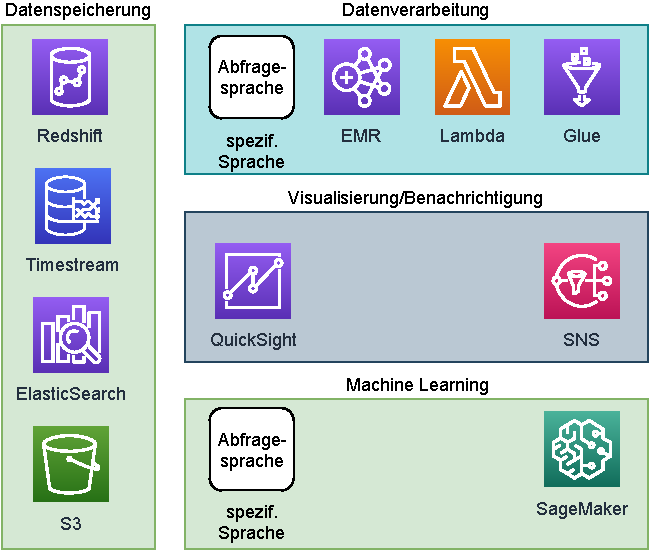
\includegraphics[width=\textwidth]{graphics/Overview-DB.pdf}
\caption{Einsetzbare Dienste im Bereich Datenbankverarbeitung}
\label{abb:ProdukteDB}
\end{figure}

\subsection{Amazon Timestream}
Timestream ist nach Aussage des Herstellers eine schnelle, skalierbare und speziell für Zeitreihendaten entwickelte Datenbank, welche über \ac{AWS} als Dienstleistung bezogen werden kann.\footcite[Vgl. auch im Folgenden][]{AmazonWebServicesInc..o.J.h} Timestream integriert zwei verschiedene Speichertypen, nämlich \ac{RAM}-basierten Speicher, in dem Daten, auf welche schnell zugegriffen werden sollen, gespeichert werden können, und Festplatten-basierten Speicher, welcher für historische Daten dienen soll.
Timestream besitzt zusätzlich einen eigenen \ac{SQL}-Dialekt, welcher um Funktionen zur Analyse von Zeitreihendaten erweitert wurde. 

Timestream ist nicht selbst in der Lage, Abfragen zu planen. \ac{AWS} gibt in der Dokumentation an, dass Lambda verwendet werden kann, um periodisch eine Abfrage in Timestream auszuführen und basierend auf dieser Anfrage Alarme via \ac{SNS} zu versenden.\footcite[Vgl.][]{AmazonWebServicesInc..o.J.ag} Abgebildet ist diese Interaktion in \autoref{abb:TimestreamLambdaOrchestration}.


\begin{figure}[H]
\centering
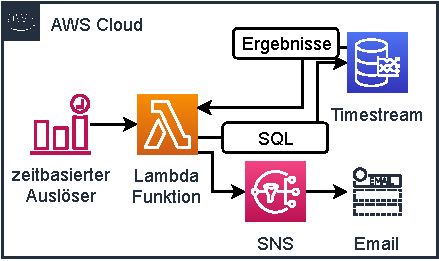
\includegraphics[width=0.45\textwidth]{graphics/Lambda-Timestream-Orchestration.pdf}
\caption{Orchestrierung von zeitbasierten Timestream Abfragen}
\label{abb:TimestreamLambdaOrchestration}
\end{figure}

\miniabschnitt{Gesamtkosten}
Timestream ist momentan noch nicht in Frankfurt verfügbar, weshalb die Kosten in der einzigen europäischen Zone mit verfügbarem Timestream, Irland, als Maßstab verwendet werden. Angenommen wird, dass die Daten eine Stunde im \ac{RAM} vorgehalten werden und danach in die Festplattenspeicherung überführt werden.

Ausgehend von dem beschriebenen Szenario lässt sich nicht genau errechnen, welche Datenmenge von den Anfragen genau erfasst wird. Dies ist dem Fakt geschuldet, dass Timestream die Daten optimiert abspeichert und nur den tatsächlichen Messwert speichert. Numerische Daten können als 32bit int, als 64bit BigInt oder als 64bit double gespeichert werden.\footcite[Vgl. auch im Folgenden][]{AmazonWebServicesInc..o.J.r}\nzitat\footcite[Vgl. auch im Folgenden][]{AmazonWebServicesInc..o.J.q} Wenn dazu ein String für die Sensorid im Stile \enquote{Sensor-123} angenommen wird, der 19 bytes zur Darstellung benötigt und der Zeitstempel addiert wird, der 8 bytes benötigt, ergibt sich eine Speicherbelegung von 91 bytes. Speicherkosten werden aber bei Werten unter einem Kilobyte auf einen Kilobyte hochgerundet, weshalb dies in der Speicherrechnung keine Beachtung findet. Wenn weitere Optimierungen, die die Abfrageengine macht, außer Acht gelassen werden, muss mit 0,78624GB pro abgefragtem Monat gerechnet werden.


\begin{table}[H]
\centering
\begin{tabular}{|l|l|l|}
\hline
Dimension & Preis(\$)/Einheit & Summe (\$) \\ \hline
Schreibzugriffe & 0,5654/Mio./KB & 4,8851 \\ \hline
\begin{tabular}[c]{@{}l@{}}\ac{RAM} \\ Speicherung\end{tabular} & 0,0407/GB/h & 0,3516 \\ \hline
\begin{tabular}[c]{@{}l@{}}Festplatten\\ Speicherung\end{tabular} & 0,0339/GB/Monat & 0,8787 \\ \hline
Anfragen & \begin{tabular}[c]{@{}l@{}}0,011308/GB \\ abgefragt\end{tabular} & 25,6055 \\ \hline
Step Functions & \begin{tabular}[c]{@{}l@{}}0,025/1000 \\ Zustandsübergänge\end{tabular} &  1,08\\ \hline
Lambda Ausführungen & 0,0000002/Ausführung & 0,0002 \\ \hline
Lambda \ac{RAM} & 0,0000000167/GB-Sekunde & 0,08 \\ \hline
\ac{SNS} (Push) & \begin{tabular}[c]{@{}l@{}}0,00002/Nachricht\\ (angenommen 5 Alarme/Gerät/Monat)\end{tabular} & 0,02 \\ \hline
Summe & \cellcolor[HTML]{EFEFEF} & 32,9011 \\ \hline
\end{tabular}
\caption{Kostenvergleich AWS~Timestream}
\label{tab:kostenvergleich-AWS~Timestream}
\end{table}


\weitereevaluationen{Amazon~Timestream}

\subsection{Amazon Athena/Amazon S3}\label{chap:athena}
Amazon Athena ist nach Aussage des Herstellers ein voll verwalteter Query Dienst, welcher das Durchsuchen von großen Datenmengen im \ac{S3} Speicherdienst möglich macht.\footcite[Vgl.][]{Barr.2016} Athena basiert dabei auf dem ursprünglich von Facebook entwickelten Presto, welches mittlerweile Open Source ist. Innerhalb von Athena können Daten verschiedener Formate (\ac{CSV}, Apache Parquet, Apache ORC, \ac{JSON}, ...) mittels \ac{SQL} verarbeitet werden. Zusätzlich ist seit November 2020 mittels der sogenannten \enquote{Federated Queries} auch die Abfrage von anderen Datenquellen wie Apache HBase, Amazon DocumentDB oder von Datenquellen, die durch eigen entwickelte Verbindungselemente verknüpft werden.\footcite[Vgl.][]{AmazonWebServicesInc..o.J.s} Technisch werden diese Federated Queries via Lambda abgewickelt.

\begin{figure}[H]
\centering
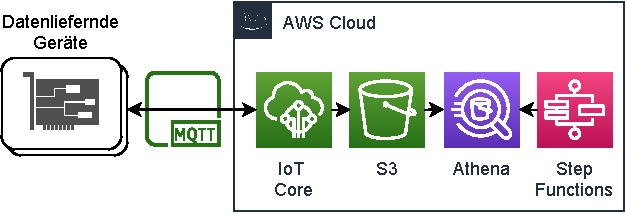
\includegraphics[width=0.8\textwidth]{graphics/Athena-general.pdf}
\caption{Grobarchitektur des Ablaufes für Athena}
\label{abb:GrobArchitekturAthena}
\end{figure}

In \autoref{abb:GrobArchitekturAthena} wird die Grobarchitektur unter Einsatz von \AWSIOT{} Core, \ac{S3}, Athena und StepFunctions gezeigt. StepFunctions dient als Orchestrierungsdienst, für die wiederholte Ausführung der Abfragen und entsprechende Weiterleitung an \ac{SNS}.
Bei verändernden Datenschemata wird empfohlen, den Dienst \ac{AWS} Glue Crawler komplementär einzusetzen, welcher die Schemata aus \ac{S3} automatisch extrahiert und in Athena hinterlegt. Andernfalls können die Schemata auch manuell hinterlegt werden.


\miniabschnitt{Gesamtkosten}
Für die folgende Kostenbewertung wird angenommen, dass Athena die Daten aus \ac{S3} indiziert. Dort liegen die Daten im \ac{JSON} Format gespeichert vor. Zu beachten ist, dass effizientere Formate wie CSV, oder sogar Apache Parquet und ORC verfügbar sind. Diese können komprimiert Daten speichern. Eine Verwendung von Parquet oder ORC würde laut \ac{AWS} 30-90\% Kosten sparen.\footcite[Vgl.][]{AmazonWebServicesInc..o.J.t} Gleichzeitig kann aber eine Speicherung im \ac{JSON} Format via \AWSIOT{} Rule erfolgen, ohne dass weitere Verarbeitung notwendig ist.

In \autoref{tab:kostenvergleich-Amazon~Athena} wird davon ausgegangen, dass 2MB an Daten im Zeitraum von 10 Minuten neu hinzukommen. Da aber eine Historie gebildet werden soll, müssen sowieso die gesamten dreimonatigen historischen Daten abgefragt werden. Ausgehend von 200 kB pro Minute von allen Geräten ergeben sich 25,92 GB \ac{S3}-Datenvolumen an historischen Daten, welche 960 mal im Monat abgefragt werden sollen. Athena rundet dabei auf das nächste MegaByte auf und hat ein Minimum von 10 MB erfasster Daten pro Anfrage.\footcite[Vgl.][]{AmazonWebServicesInc..o.J.t} Das Datenschema für Athena stellt Glue bereit, welches Kosten für Abfragen aus dem Datenkatalog und Speicherkosten für den Datenkatalog erhebt.\footcite[Vgl.][]{AmazonWebServicesInc..o.J.u} Zur Orchestrierung wird ein Ablauf als Zustandsmaschine in StepFunctions abgebildet, welches für jeden Zustandsübergang eine Gebühr erhebt.\footcite[Vgl.][]{AmazonWebServicesInc..o.J.v}

\begin{table}[H]
\centering
\begin{tabular}{|l|l|l|}
\hline
Dimension & Preis(\$)/Einheit & Summe (\$) \\ \hline
Athena Abfragen & \begin{tabular}[c]{@{}l@{}}0,005/TB \\ abgefragte Daten\end{tabular} &  121,50\\ \hline
\ac{S3}-Speicher & 0,0245/GB Speicher & 0,64 \\ \hline
\begin{tabular}[c]{@{}l@{}}Glue Data Catalog\\ Speicher\end{tabular} & 1/100.000 Objekte &  \textless 0,0001\\ \hline
\begin{tabular}[c]{@{}l@{}}Glue Data Catalog\\ Abfragen\end{tabular} & 1/Million Abfragen &  \textless 0,0001\\ \hline
Step Functions & \begin{tabular}[c]{@{}l@{}}0,025/1000 \\ Zustandsübergänge\end{tabular} &  1,08\\ \hline
\ac{SNS} (Push) & \begin{tabular}[c]{@{}l@{}}0,00002/Nachricht\\ (angenommen 5 Alarme/Gerät/Monat)\end{tabular} & 0,02 \\ \hline
Summe & \cellcolor[HTML]{EFEFEF} &  123,24\\ \hline
\end{tabular}
\caption{Kostenvergleich Amazon~Athena}
\label{tab:kostenvergleich-Amazon~Athena}
\end{table}

\weitereevaluationen{Amazon~Athena/Amazon~S3}


\subsection{Amazon Redshift}

Amazon Redshift ist der Data Warehouse Dienst von \ac{AWS}, welcher nach Aussage des Herstellers \enquote{enterprise-level} ist und auf ein Datenvolumen von Petabytes skalieren kann. \footcite[Vgl.][1]{AmazonWebServicesInc..o.J.g} Redshift ist dabei ein klassischer \ac{OLAP} Dienst, welcher für eine Vielzahl verschiedener Daten effizient Auswertungen bereitstellen kann. Redshift basiert auf der bekannten Open Source Datenbank PostgreSQL, weicht jedoch in der Implementierung diverser Kommandos und Features ab, die Amazon für irrelevant bei \ac{OLAP} Anwendungen hält.\footcite[Vgl.][4]{AmazonWebServicesInc..o.J.g}\nzitat\footcite[Vgl.][428\psqq]{AmazonWebServicesInc..o.J.g} Kern von Redshift sind sogenannte Cluster, welche aus einem oder mehreren Berechnungsknoten (\enquote{compute nodes}) und Anführerknoten (\enquote{leader nodes}) bestehen. Applikationen interagieren allein mit den Anführerknoten, die existierenden Berechnungsknoten sind zwar transparent für die Anwendung, werden jedoch von den Anführerknoten mit Ausführungsplänen versorgt, die diese entwickelt, um Anfragen effizient zu verarbeiten.\footcite[Vgl.][4]{AmazonWebServicesInc..o.J.g}

Redshift bietet zusätzlich mit Redshift Spectrum einen Dienst an, welcher auf den ersten Blick dem in \autoref{chap:athena} vorgestellten Athena gleicht. Beide rufen via \ac{SQL} Daten von \ac{S3} ab und beide kosten 5\$/TB gescannte Daten.\footcite[Vgl. auch im Folgenden][]{Smallcombe.2020} Wichtige Unterschiede liegen dabei aber in der Art, wie Ressourcen verwaltet und genutzt werden können. Während Redshifft Spectrum nur in Kombination mit einem Redshift Cluster verwendet werden kann, funktioniert Athena ohne Kopplung an verwaltende Ressourcen. Gleichzeitig ist ein stärkerer Einfluss auf die Performance bei Redshift möglich, da zusätzliche Clusterressourcen einfach provisionierbar sind, während Athena vollständig von \ac{AWS} verwaltet wird. Entsprechend erlaubt Redshift Spectrum zwar größeren Einfluss auf die Performance von Datenabfragen, dieser Einfluss muss jedoch in Form von zusätzlich abzurechnenden Clusterressourcen abgerechnet werden, was Redshift für Anwendungsfälle, die keine gesichert gleichbleibende Performance benötigen, unattraktiv macht.

\begin{figure}[H]
\centering
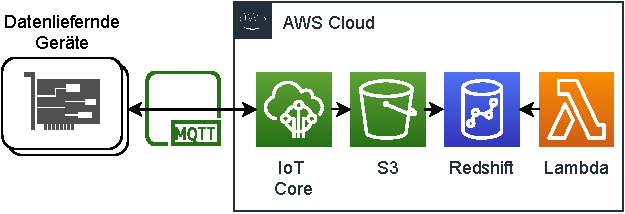
\includegraphics[width=0.8\textwidth]{graphics/Redshift-general.pdf}
\caption{Grobarchitektur des Ablaufes für Redshift}
\label{abb:GrobArchitekturRedshift}
\end{figure}

In \autoref{abb:GrobArchitekturRedshift} ist beispielhaft die Verwendung von Redshift mit \ac{S3} (ohne Spectrum) gezeigt. Dabei lädt Redshift die Daten von \ac{S3} und löscht diese anschliessend. Anfragen werden via der \ac{JDBC}-Schnittstelle von Redshift mit Lambda getätigt und ausgewertet. Alternativ könnte Kinesis Data Firehose zum Laden der Daten in Redshift zum Einsatz kommen.


\miniabschnitt{Gesamtkosten}
Im Vergleich von \citeauthor{Gupta.2015}, bei dem alle Autoren \ac{AWS} angehören, bescheinigen sie Redshift ein \enquote{disruptives} Preismodell gegenüber anderer DataWarehouse Lösungen.\footcite[Vgl.][]{Gupta.2015} Ob für den Usecase dieser Arbeit Redshift ebenfalls ein \enquote{disruptives} und ansprechendes Preismodell hat, soll im Folgenden erläutert werden.

Da Redshift Spectrum durch die zusätzlich zu provisionierenden Clusterresourcen einen Kostennachteil hat, wie auch von \citeauthor{Tan.2019} festgestellt, wird von einem Kostenvergleich für Spectrum abgesehen.\footcite[Vgl.][2178]{Tan.2019}

Stattdessen werden die Kosten für ein \enquote{shared-nothing}\footcite[Vgl.][2172]{Tan.2019} Redshift \ac{OLAP} Cluster berrechnet. Dabei ist zu beachten, dass \AWSIOT{} keine direkte Regel bietet, um Daten in Redshift abzulegen. Stattdessen müssen die Daten via Kinesis Data Firehose oder \ac{AWS} Lambda eingefügt werden. Zum Zwecke der Datenübertragung wird in diesem Fall Kinesis Data Firehose kalkuliert. Wie bei Elasticsearch Service gibt es auch bei Redshift verschiedene unterliegende Instanzen zur Auswahl.\footcite[Vgl. auch im Folgenden][]{AmazonWebServicesInc..o.J.z} Im Vergleich werden, den Empfehlungen von \ac{AWS} folgend, eine Instanz der \ac{DC2} Klasse verwendet, welche sich für unkomprimierte Datenmengen kleiner ein TB eignen. Die kleinste verfügbare \ac{DC2} Instanz ist \enquote{dc2.large} mit 2 vCPUs, 15GiB Hauptspeicher und ~160 GB Festplattenspeicher. Redshift muss innerhalb eines \acp{VPC} gestartet werden, um Netzwerkisolation sicherzustellen. Aus diesem Grund ist ein Aufpreis auf Kinesis Data Firehose zu zahlen, welches Datenübertragung in ein \ac{VPC} mit einem Aufschlag berechnet.\footcite[Vgl. auch im Folgenden][]{AmazonWebServicesInc..o.J.y} Kinesis Data Firehose rundet dazu noch Daten zu den nächsten 5 KB auf, was eine effektive Datenmenge von 41,77GB ergibt.

Um Alarme an \ac{SNS} zu übermitteln, müssen Anfragen mittels einer Lambdafunktion orchestriert werden. Diese Funktion wertet die Resultate der Anfragen aus und schickt darauf basierend Alarme. Entsprechend müssen die Kosten für Lambda und \ac{SNS} eingerechnet werden.\footcite[Vgl.][]{AmazonWebServicesInc..o.J.bx}\nzitat\footcite[Vgl.][]{AmazonWebServicesInc..o.J.by}

\begin{table}[H]
\centering
\begin{tabular}{|l|l|l|}
\hline
Dimension & Preis(\$)/Einheit & Summe (\$) \\ \hline
\begin{tabular}[c]{@{}l@{}}dc2.large Instanz\\ (OnDemand)\end{tabular} & 0,324/h & 233,60 \\ \hline
\begin{tabular}[c]{@{}l@{}}Firehose \\ Dateneingang\end{tabular} & 0,033/GB & 1,38 \\ \hline
\begin{tabular}[c]{@{}l@{}}Firehose\\ \ac{VPC}\end{tabular} & \begin{tabular}[c]{@{}l@{}}0,01/GB\\ 0,012/h\end{tabular} & 8,84 \\ \hline
Lambda Ausführungen & 0,0000002/Ausführung & 0,000192 \\ \hline
Lambda \ac{RAM} & 0,0000000167/GB-Sekunde & 0,08 \\ \hline
\ac{SNS} (Push) & \begin{tabular}[c]{@{}l@{}}0,00002/Nachricht\\ (angenommen 5 Alarme/Gerät/Monat)\end{tabular} & 0,02 \\ \hline
Summe & \cellcolor[HTML]{EFEFEF} & 243,920192 \\ \hline
\end{tabular}
\caption{Kostenvergleich Amazon~Redshift}
\label{tab:kostenvergleich-Amazon~Redshift}
\end{table}

\weitereevaluationen{Amazon~Redshift}

\subsection{Amazon OpenSearch Service}

Amazon OpenSearch Service ist die verwaltetete Variante des Elasticsearch Forks von Amazon, OpenSearch.\footcite[Vgl. auch im Folgenden][]{Meadows.2021} OpenSearch Service, dessen Namensänderung weg von Elasticsearch Service im April 2021 angekündigt wurde, bietet die Datenbank Elasticsearch als Service an, welche ursprünglich von Elastic entwickelt wurde. Elasticsearch ist dabei nach Aussage des Herstellers eine verteilte, freie und offene Analytics- und Suchplattform für viele verschiedenen Datenformen.\footcite[Vgl.][]{ElasticsearchInc..o.J.} Elasticsearch basiert auf der Open Source Bibliothek Apache Lucene, welche besonders für Suchabfragen in großen Datenmengen optimiert ist. Elasticsearch ist neben Anwendungsfällen im Bereich Logverarbeitung und Monitoring auch für \ac{IIoT} Anwendungsfälle bekannt.\footcite[Vgl.][]{Mantfeld.2019}\nzitat\footcite[Vgl.][]{Bajer.2017}

\begin{figure}[H]
\centering
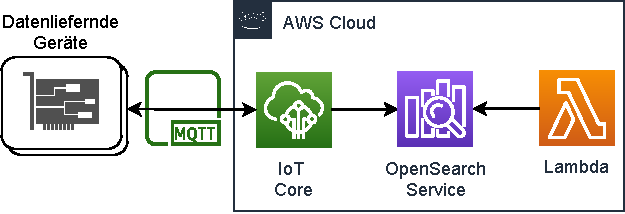
\includegraphics[width=0.8\textwidth]{graphics/OpenSearch-general.pdf}
\caption{Grobarchitektur des Ablaufes für OpenSearch Service}
\label{abb:GrobArchitekturOpenSearch}
\end{figure}
Wie in \autoref{abb:GrobArchitekturOpenSearch} gezeigt, kann OpenSearch/Elasticsearch Service nativ via \AWSIOT{} Core Daten empfangen. Lambda dient zur Orchestrierung der Abfragen und zur folgenden Auswertung.

\miniabschnitt{Gesamtkosten}
Der \ac{AWS} OpenSearch Service wird auf unterliegenden \ac{EC2} Instanzen betrieben und wie diese in gewissen Klassen abgerechnet. Dabei stehen sowohl OnDemand Abrechnugsmodelle wie auch reservierte Kapazität zur Verfügung.\footcite[Vgl. auch im Folgenden][]{AmazonWebServicesInc..o.J.w} Zusätzlich steht mit \enquote{UltraWarm} eine besondere Instanzklasse zur Verfügung, welche für das Vorhalten großer Datenmengen konzipiert ist. Zusätzlich zu den Instanzen wird noch der verbrauchte \ac{EBS}-Speicherplatz abgerechnet. Dieser Speicherplatz kann in der Standard Klasse oder speziell für hohen Datendurchsatz (provisionierte \ac{IOPS}) gebucht werden. Der Speicherplatz für UltraWarm wird aber nicht via \ac{EBS} abgerechnet, sondern separat. Ebenfalls steht wieder ein \enquote{Free Tier} zur Verfügung, welches aus Vergleichsgründen nicht in die Berechnung einfliessen soll. Aus Vergleichsgründen kommen nur OnDemand abgerechnete Instanzen für den Vergleich in Frage. Für Vergleichszwecke soll eine t3.medium.elasticsearch Instanz geschätzt werden, welche mit 2 vCPUs und 4 GiB \ac{RAM} ausgestattet ist. Der provisionierte \ac{EBS}-Speicherplatz soll bei 10GB liegen.
Benachrichtigungen werden über die native Integration von Kibana (Name nach Umbenennung: OpenSearch Dashboards) und \ac{SNS} abgewickelt, wobei Kibana die Wertüberwachung übernimmt.\footcite[Vgl.][]{AmazonWebServicesInc..o.J.x}

\begin{table}[H]
\centering
\begin{tabular}{|l|l|l|}
\hline
Dimension & Preis(\$)/Einheit & Summe (\$) \\ \hline
\begin{tabular}[c]{@{}l@{}}t3.medium Instanz\\ (OnDemand)\end{tabular} & 0,084/h & 61,32 \\ \hline
\ac{EBS} Speicher & 0,161/GB & 1,61 \\ \hline
\ac{SNS} (Push) & \begin{tabular}[c]{@{}l@{}}0,00002/Nachricht\\ (angenommen 5 Alarme/Gerät/Monat)\end{tabular} & 0,02 \\ \hline
Summe & \cellcolor[HTML]{EFEFEF} & 62,95\\ \hline
\end{tabular}
\caption{Kostenvergleich Amazon~OpenSearch~Service}
\label{tab:kostenvergleich-Amazon~Elasticsearch~Service}
\end{table}

\weitereevaluationen{Amazon~OpenSearch~Service}

\subsection{Auswahl}
Folgend werden die einzelnen Dienste anhand der in \autoref{tab:umfragen-auswertungen} priorisierten Kriterien bewertet.
\begin{table}[H]
    \centering
    \begin{tabular}{|l|l!{\vrule width 2pt}l|l|l|l|}
    \hline
\multicolumn{1}{|c|}{Kriterium} & \multicolumn{1}{c!{\vrule width 2pt}}{\begin{tabular}[c]{@{}c@{}}max.\\Punkte\end{tabular}} & \multicolumn{1}{c|}{\begin{tabular}[c]{@{}c@{}}Amazon\\Timestream\end{tabular}} & \multicolumn{1}{c|}{\begin{tabular}[c]{@{}c@{}}Amazon\\OpenSearch\end{tabular}} & \multicolumn{1}{c|}{\begin{tabular}[c]{@{}c@{}}Amazon\\Athena\end{tabular}} & \multicolumn{1}{c|}{\begin{tabular}[c]{@{}c@{}}Amazon\\Redshift\end{tabular}} \\ \hline
     \begin{tabular}[c]{@{}l@{}}Übertragbarkeit zwischen \\ Clouds (ISO 9126)\end{tabular} & 1 & 0 & 1 & 1 & 0 \\ \hline
     \begin{tabular}[c]{@{}l@{}}Integration mit anderen \\ \ac{AWS} Diensleistungen\end{tabular} & 3 & 3 & 3 & 3 & 3 \\ \hline
     Generalisierung & 4 & 4 & 4 & 4 & 4 \\ \hline
     Erweiterbarkeit & 4 & 4 & 4 & 4 & 4 \\ \hline
     \begin{tabular}[c]{@{}l@{}}Fehlertransparenz/ \\ Debugability\end{tabular} & 5 & 5 & 5 & 4 & 5 \\ \hline
     \begin{tabular}[c]{@{}l@{}}geringer \\ Wartungsaufwand\end{tabular} & 7 & 7 & 5 & 7 & 5 \\ \hline
     \begin{tabular}[c]{@{}l@{}}Skalierbarkeit \& \\ \enquote{serverlessness}\end{tabular} & 7 & 7 & 5 & 7 & 5 \\ \hline
     Kosten & 7 & 7 & 6 & 5 & 4 \\ \hline
     Performancegarantien & 8 & 8 & 8 & 8 & 8 \\ \hline
     \begin{tabular}[c]{@{}l@{}}Robustheit \& \\ Fehlertoleranz\end{tabular} & 9 & 9 & 9 & 6 & 9 \\ \hline
     \begin{tabular}[c]{@{}l@{}}Auswertungen \\ (\autoref{chap:auswertungsarten}) \end{tabular} & 11 & 11 & 11 & 11 & 11 \\ \hlinewd{2pt}
     \rowcolor[HTML]{ECF4FF}
     Summe & 66 & \textbf{\cellcolor[HTML]{ECF4FF}65} & \textbf{\cellcolor[HTML]{ECF4FF}61} & \textbf{\cellcolor[HTML]{ECF4FF}60} & \textbf{\cellcolor[HTML]{ECF4FF}58} \\ \hline
\end{tabular}
\caption{Bewertungsmatrix~Batch}
\label{tab:bewertungsmatrix-batch}
\end{table}

\miniabschnitt{Übertragbarkeit zwischen Clouds}
Übertragbare Dienste/Produkte sind Amazon OpenSearch und Amazon Athena. OpenSearch, welches größtenteils Kompatibilität zu ElasticSearch hat (mit Ausnahme des Amazon eigenen Anomalieeerkennungsplugins), kann mit Anpassungen mit dem ElasticSearch Code in anderen Public Clouds verwendet werden. Da Athena auf Presto basiert, sind Abfragen kompatibel und portabel. Dies erfordert entsprechende Unterstützung für Presto in der Zielcloud oder eine eigene Installation.

\miniabschnitt{Integration mit AWS}
Bei den verglichenen Diensten handelt es sich mit Ausnahme von OpenSearch um von Amazon teilweise oder komplett entwickelte properitäre Dienste, weshalb die Integration mit anderen \ac{AWS} Dienstleistungen gegeben ist. Auch OpenSearch wird mittlerweile, als Fork von Elasticsearch, hauptsächlich von \ac{AWS} betreut und ist bereits gut mit anderen Dienstleistungen integriert.

\miniabschnitt{Generalisierung}
Alle betrachteten Systeme sind fähig generalisierte Usecases mit Zeitreihen abzubilden. Abseits von Zeitreihen wäre Timestream im Vergleich zu den anderen Diensten eher ungeeignet, dies ist aber nicht im Themenfokus der Arbeit. 

\miniabschnitt{Erweiterbarkeit}
Auch wenn die verglichenen Datenbankdienste für jeweils individuelle Zwecke entwickelt wurden, sind sie doch generalisiert für mehrere Usecases verwendbar und erweiterbar.

\miniabschnitt{Fehlertransparenz}
Im Bereich Fehlertransparenz gab es Abzug für Athena, da fehlschlagende Abfragen nur mit generischen Fehlermeldungen beantwortet werden, was die Fehlersuche erschwert.\footcite[Vgl.][]{Cooney.2020}

\miniabschnitt{Geringer Wartungsaufwand}
Punktabzüge im Wartungsaufwand und der Skalierbarkeit gab es für die auf Instanzen basierenden Dienste OpenSearch und Redshift, welche durch die von Nutzenden vorzunehmende vertikale Skalierung einen höheren Wartungs- und Überprüfungsaufwand fordern, als Timestream und Athena, die verwaltet sind.

\miniabschnitt{Skalierbarkeit \& serverlessness}
Abzüge für die Skalierbarkeit gab es für beide instanzbasierten Dienste, OpenSearch und Redshift, welche nicht in der Geschwindigkeit wie serverless Dienste skaliert werden können.

\miniabschnitt{Kosten}
Der von \citeauthor{Tan.2019} konstatierte Preisvorteil von Redshift gegenüber Athena hat sich in dem durchgeführten Vergleich nicht gezeigt.\footcite[Vgl.][2178\psq]{Tan.2019} Dies könnte womöglich dem Fakt geschuldet sein, dass die Datenmengen der Studie einen \enquote{Break-even} Punkt überschritten haben, an dem das Athena Abrechnungsmodell im Vorteil gegenüber Redshift war.
Die Gesamtkosten scheinen bei Redshift zumindest im vorliegenden Fall, ohne konkrete Optimierungen, besonders hoch zu sein, genauso wie bei Athena. Kostenführer ist Timestream, gefolgt von OpenSearch Service. Da Timestream basierend auf tatsächlichem Verbrauch an Speicher und abgefragter Datenmenge abrechnet, führt Timestream die Kategorie Kosten an.

\miniabschnitt{Performancegarantien}
Die Performance der verglichenen Dienste variierte aufgrund verschiedener unterliegender Faktoren, wie beispielsweise provisionierter Leistung oder der Optimierung für spezifische Anfragen, was andere Anfragen verlangsamte. Letzten Endes ist es fraglich, ob \ac{OLAP} Analysen, die zeitgesteuert erstellt werden, eine garantierte Performance im Sub-Sekunden Bereich brauchen, oder ob es reicht, die Analyse in längerer Zeit zu erledigen, da die Daten sowieso zeitversetzt sind.
Alle verglichenen Dienste können die Auswertungen in angemessener Zeit anfertigen. 

\miniabschnitt{Robustheit \& Fehlertoleranz}
Athena hat Punktabzüge im Bereich Robustheit \& Fehlertoleranz, da ein sich veränderndes Datenschema zu schwerwiegenderen Problemen führen kann.

\miniabschnitt{Auswertungen}
Alle Dienste bieten die gewünschten Auswertungen an. Technisch sind aufgrund der unterschiedliche Implementierungen trotzdem Unterschiede vorhanden. 

\miniabschnitt{Conclusio}
Im Vergleich hat Timestream am besten abgeschnitten, gefolgt von OpenSearch. Timestream erhielt Punktabzug aufgrund der fehlenden Übertragbarkeit zwischen Clouds, über die OpenSearch/Elasticsearch als zweite Wahl verfügt. Im Gegensatz zur zweiten Wahl ist Timestream dabei vollständig verwaltet und skaliert ohne Interaktion von Nutzenden, was sowohl den Wartungsaufwand verringert, als auch das Kriterium Skalierbarkeit besser erfüllt. 





